\chapter{Componente Processor Expert}

\section{Porturi de intrare și ieșire}
Cu ajutorul componentei \textit{BitIO} din Processor Expert putem accesa porturi de intrare și iesire ale microcontrollerului, folosind pinii configurabili ai acestuia. O astfel de componentă este caracterizată de un nume, de un pin al microcontrollerului pe care este mapată, o direcție (portul poate fi de intrare sau de ieșire) și valoarea inițiala, în cazul pinilor configurați pentru ieșire. 

\begin{figure}[h!]
  \vspace{-20pt}
  \center{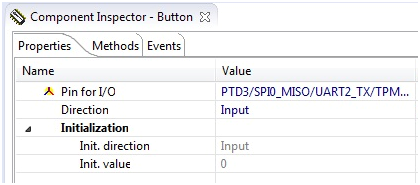
\includegraphics[width=0.5 \textwidth]{images/BitIO.png}}
  \vspace{-15pt}
  \caption{\label{fig:CodeWarrior-BitIO} Configurarea unui port de intrare / ieșire}
  \vspace{-20pt}
\end{figure}